%!TEX root =  ../main.tex
\renewcommand{\columnseprule}{1.5pt}
\begin{multicols*}{2}
\rule[0.5\baselineskip]{0.4\textwidth}{1pt}
\noindent
\LabSection{Magic Number}\label{sec:0801p}
\begin{exercises}{sec:0801p}
\lab{} \textbf{Magic number}  We posit that there is at least one simple exponential function whose height at any given point is also equal to its derivative at that point.  Sketch a graph of an un-translated exponential function, without a grapher, of the form $f(x)=Ax$.  Label the y-intercept all such graphs have in common.

\vspace{4cm}
\lab{}  Rather than dealing within further math, let us choose the easiest point for the algebra.  Work out the derivative formula for $f(x)$ at 0.  Rather than taking the limit, leave h in the equation.  Record it below.

\vspace{3cm}
\lab{} Calculate the approximate derivative for several values of $A$, using an $h$ of $10^{-8}$ or smaller.  Guess-and-check until you get a derivative of 1.000.  What must $A$ be?

\vspace{3cm}
\lab{} Graph your $f(x)=Ax$ and its tangent line through (0,1).

\noindent
\begin{centering}
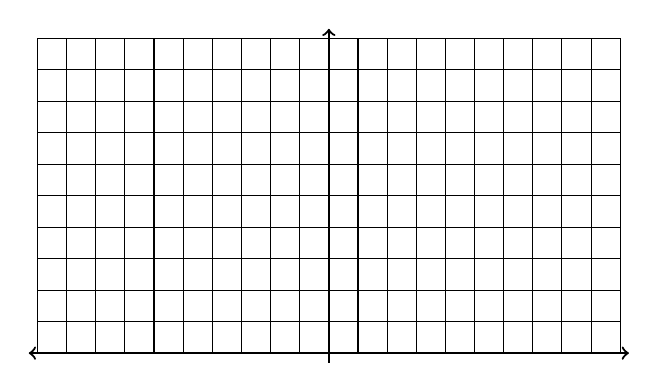
\begin{tikzpicture}[xscale=0.37,yscale=0.04]
	\draw [thick, <->] (-10.3,0) -- (10.3,0);
	\draw [thick, ->] (0,-3) -- (0,103);
	\draw [thin,ystep=10] (-10,0) grid (10,100);
\end{tikzpicture}
\end{centering}

\lab \textbf{Another Magic Number}  What is the most amount of money you could get out of a bank in a year?  Suppose you invested a \$1.00 and got 100\% interest.  How much would you have at the end of the year?


\vspace{1cm}
\lab{} Now suppose you asked them instead to compound your interest twice in a year.  (This means they give you 50\% interest each time.)  How much would you have at the end of such a year?

\vspace{1cm}
\lab{} That went so well, you decide to see how far you take this.  How much does 100\%$\div 4$, compounded 4 times a year get you?

\vspace{2cm}
\lab{} Write a formula and take the limit as the number of time interest is compound goes to infinity.  What is the theoretical maximum you could make from a bank willing to compound continuously?

\vspace{2cm}
\lab{} The magic number you found twice is called $e$, and is as important in calculus as $\pi$ is in geometry.  Find another definition of $e$.

\vspace{2cm}
\lab{} Describe in your own word what you think the point of this problem set is.

\end{exercises}
\end{multicols*}